%%%%%%%%%%%%%%%%%%%%%%%%%%%%%%%
% Thesis/dissertation template
%   Department of Logistics
%   Stellenbosch University
%%%%%%%%%%%%%%%%%%%%%%%%%%%%%%%
\documentclass[serif,11pt]{beamer}
\usepackage[ruled, linesnumbered,vlined]{algorithm2e}
\usepackage{epsfig, subfigure, amssymb, multirow, algorithmic,amsmath}
\usetheme{Warsaw}
\usepackage{multirow}
\newcommand*{\superscript}[1]{\ensuremath{^{\rm #1}}}
\newcommand*{\subscript}[1]{\ensuremath{_{\rm #1}}}

%%%%%%%%%%%%%%%%%%
%
% thesis details
%
%%%%%%%%%%%%%%%%%%

\begin{document}
\title[{\sc The short title of your thesis } \hspace{0.8cm} \insertframenumber/\inserttotalframenumber]{{\sc The title of your thesis or dissertation should be typed here }}
\author[Presentation to some students --- {\sc  May 3\superscript{rd}, 2012}]{{Student name}}
\date{3 May 2014}
\institute{Operations Research \\ in the Department of Logistics \\ University of Stellenbosch, South Africa}

\begin{frame}
\begin{center}
\vspace{0.1cm}

\includegraphics[scale=0.25]{USlogo.pdf}
\end{center}
\titlepage
\end{frame}


%%%%%%%%%%%%%%%%%%
%
% how-to examples:
%
%%%%%%%%%%%%%%%%%%

\begin{frame}\frametitle{Overview}
\begin{itemize}
\pause \item The trivial Set Cover algorithm has running time of ${\cal O}(2^n)$.
\pause \item bla, bla, bla\ldots
\end{itemize}

\end{frame}

\begin{frame}\frametitle{Domination on a Chessboard}
\begin{figure}[htb]
\centering
 \begin{tabular}{cc}\pause{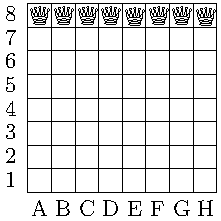
\includegraphics[scale=1]{examples/DomChess8.pdf}}&
       \pause{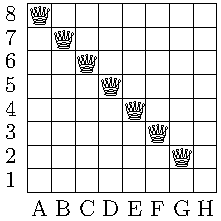
\includegraphics[scale=1]{examples/DomChess7.pdf}}\\
       \pause{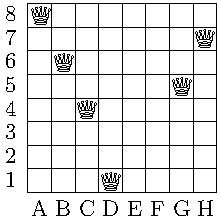
\includegraphics[scale=1]{examples/DomChess6.pdf}}&
      \pause{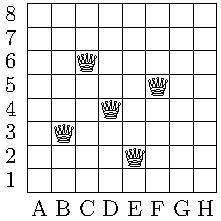
\includegraphics[scale=1]{examples/Chess1.pdf}}
      \end{tabular}
\end{figure}
\end{frame}

\SetKwInOut{Input}{Input}\SetKwInOut{Output}{Output}
\begin{frame}\frametitle{A trivial Set Cover algorithm}
\begin{algorithm}[H]\footnotesize
        \Input{A set cover instance $({\cal S,U})$ and a variable ${\cal S}_{\rm dom}$.}
        \Output{A minimum set cover of $({\cal S,U})$.}
\If{${\cal S}=\emptyset$}{
\Return $\emptyset$\;
}
Let $S \in {\cal{S}}$ be a set of maximum cardinality\;
${\cal{C}}_1 = \{S\}\cup {\tt MSC}(\{S'\backslash S \mid S' \in{\cal S}\backslash \{S\}\}, {\cal U}\backslash S )$\;
${\cal{C}}_2 = {\tt MSC}({\cal S}\backslash \{S\},{\cal U})$\;
${\cal S}_{\rm dom} \leftarrow \emptyset$\;
\If{${\cal U} \subseteq {\cal C}_1$}{
${\cal S}_{\rm dom} \leftarrow {\cal C}_1$\;
\If{${\cal U} \subseteq {\cal C}_2$}{
\If{$|{\cal C}_2| < |{\cal C}_1|$}{
${\cal S}_{\rm dom} \leftarrow {\cal C}_2$\;
}
}
}
\Return ${\cal S}_{\rm dom}$\;
\caption{{\tt MSC}$({\cal S,U})$}
\end{algorithm}
\end{frame}

%%%%%%%%%%%%%%%%%%
%
% bibliography
%
%%%%%%%%%%%%%%%%%%

\begin{frame} \frametitle{References}
\begin{thebibliography}{xx}\footnotesize

\bibitem{FominFVGrandoniFKratschD2009} {\sc Fomin FV, Grandoni F \& Kratsch D}, 2009, {\em A note on the complexity of minimum dominating set }, Journal of Discrete Algorithms, {\bf{4(2)}}, pp.\ 209--214.

\bibitem{critical} {\sc Grobler PJP \& Mynhardt CM}, 2009, {\em Secure domination critical graphs}, Discrete Mathematics, {\bf 309}, pp.~5820--5827.

\bibitem{VRB}{{\sc Van Rooij JMM \& Bodlaender HL}, 2011, {\em Exact algorithms for dominating set}, Discrete Applied Mathematics, {\bf 159}, pp.\ 2147--2164.}

\end{thebibliography}
\end{frame}

%%%%%%%%%%%%%%%%%%


\end{document}